\section{Numerical Methods}
\noindent\rule[\linienAbstand]{\linewidth}{\linienDickeDick}
\begin{equation}
  \begin{split}
    h =& t_{k+1} - t_k\\
    t_k =& t_0 + k \cdot h, \;\; k \in \mathbb{N}
  \end{split}
\end{equation}

\subsection{Explicit Eulers Method}
\noindent\rule[\linienAbstand]{\linewidth}{\linienDicke}
\begin{equation}
  \begin{split}
    x_{k+1} = x_k + h \cdot f(t_{k+1}, x_{k+1})
  \end{split}
\end{equation}

\subsection{Implizit Eulers Method}
\noindent\rule[\linienAbstand]{\linewidth}{\linienDicke}
\begin{equation}
  \begin{split}
    \dot{x} &= f(t, x)\\
    x_{k+1} &= x_k + h \cdot f(t_k, x_k)
  \end{split}
\end{equation}

\subsection{Midpoint Method}
\noindent\rule[\linienAbstand]{\linewidth}{\linienDicke}
\begin{equation}
  \begin{split}
    x_{k+\frac{1}{2}} &= x_k + \frac{h}{2} \cdot f(t_k, x_k)\\
    x_{k+1}           &= x_k + h \cdot f(t_{k} + \frac{h}{2}, x_{k+\frac{1}{2}})
  \end{split}
\end{equation}

\subsection{Heun Method}
\noindent\rule[\linienAbstand]{\linewidth}{\linienDicke}
\begin{equation}
  \begin{split}
    k_1 &= f(t_k, x_k)\\
    k_2 &= x_k + h \cdot f(t_k, x_k)\\
    x_{k+1} &= x_k + \frac{h}{2}(k_1 + k_2)
  \end{split}
\end{equation}

\subsection{Runge-Kutta Method of Fourth Order}
\noindent\rule[\linienAbstand]{\linewidth}{\linienDicke}
\begin{equation}
  \begin{split}
    k_1 &= f(t_k, x_k)\\
    k_2 &= f(t_k + \frac{h}{2}, x_k + \frac{h}{2}k_1)\\
    k_3 &= f(t_k + \frac{h}{2}, x_k + \frac{h}{2}k_2)\\
    k_4 &= f(t_k + h, x_k +h \; k_3)\\
    x_{x+1} &= x_k + \frac{h}{6}(k_1 + 2k_2 + 2k_3 + k_4)
  \end{split}
\end{equation}

\begin{figure}[H]
  \centering
  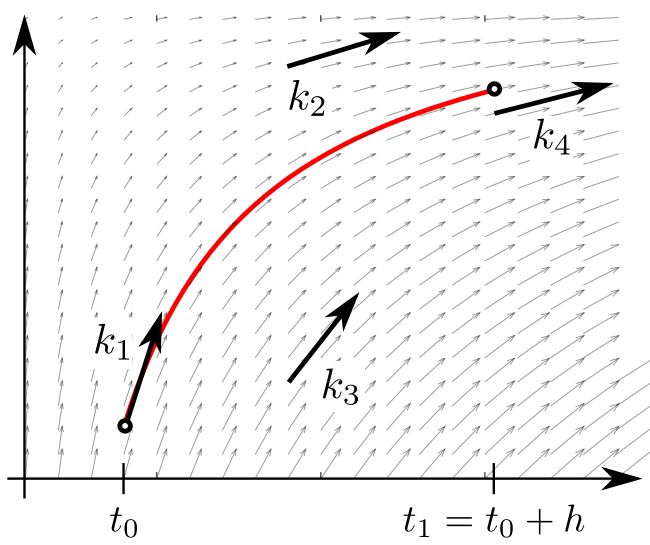
\includegraphics[width=0.5\linewidth]{Pics/runge.png}
\end{figure}

\subsection{Error Order}
\noindent\rule[\linienAbstand]{\linewidth}{\linienDicke}
The (global) error orders of the various methods discussed before are:
\begin{itemize}
  \item Explicit Euler method: $p = 1$
  \item Midpoint rule: $p = 2$
  \item Heun method: $p = 2$
  \item Classical Runge-Kutta method: $p = 4$
\end{itemize}
The higher the error order of a method, the smaller thus the error is which one has to take into account by using the method. On the other hand, the computational cost for the preciser methods is often higher as well.
